%!TEX TS-program = xelatex
%!TEX encoding = UTF-8 Unicode

\documentclass[12pt]{extarticle}
% extarticle is like article but can handle 8pt, 9pt, 10pt, 11pt, 12pt, 14pt, 17pt, and 20pt text

\def \ititle {Origins of Mind}
 
\def \isubtitle {Lecture 08}
 
\def \iauthor {Stephen A. Butterfill}
\def \iemail{s.butterfill@warwick.ac.uk}
\date{}

%for strikethrough
\usepackage[normalem]{ulem}

\input{$HOME/Documents/submissions/preamble_steve_handout}

%\bibpunct{}{}{,}{s}{}{,}  %use superscript TICS style bib
%remove hanging indent for TICS style bib
%TODO doesnt work
\setlength{\bibhang}{0em}
%\setlength{\bibsep}{0.5em}


%itemize bullet should be dash
\renewcommand{\labelitemi}{$-$}

\begin{document}

\raggedcolumns

\begin{multicols*}{3}

\setlength\footnotesep{1em}


\bibliographystyle{newapa} %apalike

%\maketitle
%\tableofcontents




%--------------- 
%--- start paste


\def \ititle {Logic I}
 
\def \isubtitle {Lecture 02}
 
\begin{center}
 
{\Large
 
\textbf{\ititle}: \isubtitle
 
}
 
 
 
\iemail %
 
\end{center}
 
Readings refer to sections of the course textbook, \emph{Language, Proof and Logic}.
 
 
 
\section{Counterexamples}
 
\emph{Reading:} §2.5
 
A \emph{counterexample} to an argument is a possible situation in which its premises are T and its conclusion F.
 
There are no counterexamples to a logically valid argument.
 
If an argument is not valid, then there is a counterexample to it.
 
To show that an argument is not logically valid, we specify a counterexample to it.
 
 
 
\section{Soundness}
 
An argument is \emph{sound} just if it is logically valid and its premises are true
 
Whether a sentence is true may change as the world changes.
 
The same applies to whether an argument is sound.
 
Whether an argument is logically valid not does change as the world changes.
 
 
 
\section{Sentence Letters}
 
\begin{center}
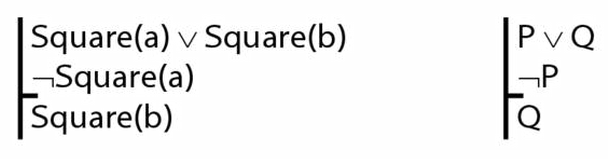
\includegraphics[scale=0.3]{img/sentence_letters.png}
\end{center}
 
 
\section{Truth Tables}
 
\emph{Reading:} §3.1, §3.2, §3.3
 
Rough guide:
 
`$\land{}$' means and
 
`$\lor{}$' means or
 
`$\lnot{}$' means not
 
\begin{center}
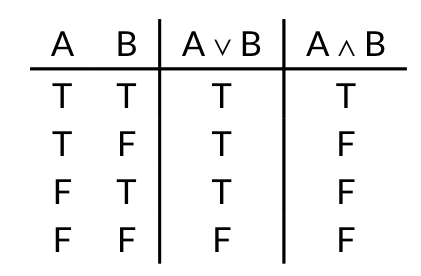
\includegraphics[scale=0.3]{img/truth_table_or_and.png}
\end{center}
\begin{center}
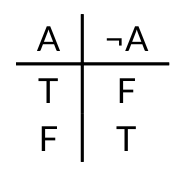
\includegraphics[scale=0.3]{img/truth_table_not.png}
\end{center}
 
 
\section{Formalizing Arguments}
 
\emph{Reading:} §3.7
 
 
 
\section{Logical Validity and Truth Tables}
 
\emph{Reading:} §4.3
 
\begin{minipage}{\columnwidth}
 
Truth tables can be used to show that an argument is valid. To illustrate ...
 
\begin{center}
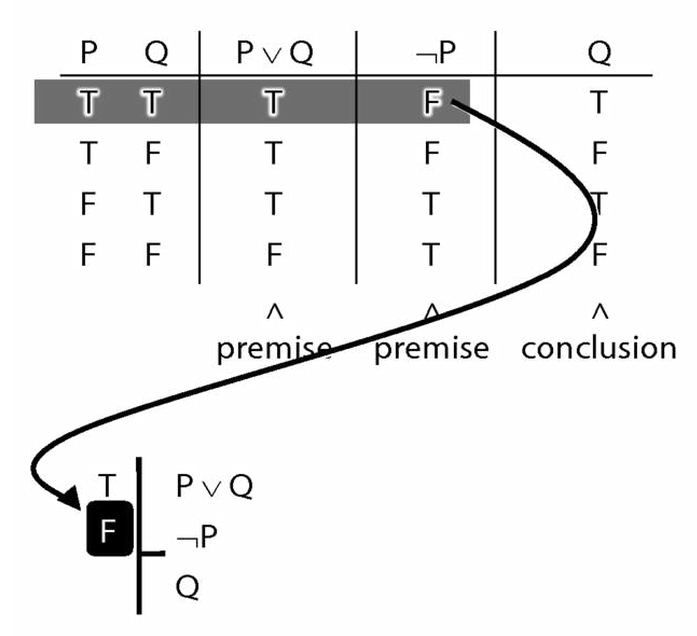
\includegraphics[scale=0.3]{img/unit_14_example.png}
\end{center}
\end{minipage}
 
\begin{minipage}{\columnwidth}
 
To establish that an argument is valid:
 
\begin{enumerate}
 
\item Create truth tables for each premise and the conclusion.
 
\item Check whether there is a row of the truth table where all premises are true and the conclusion is false.
 
\item If not, the argument is valid.
 
\end{enumerate}
 
\end{minipage}
 
 
 
\section{Complex Truth Tables}
 
\begin{center}
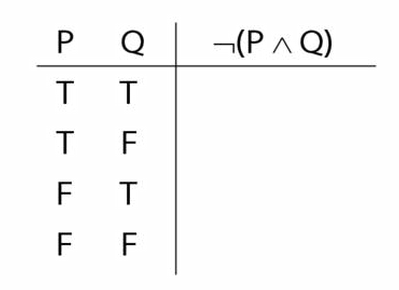
\includegraphics[scale=0.3]{img/unit_60_tt.png}
\end{center}
\vfill
\begin{minipage}{\columnwidth}
\section{Exercises}
These exercises will be discussed in seminars the week after this lecture.
The numbers below refer to the numbered exercises in the course textbook, e.g. `1.1' refers to exercise 1.1. on page 39 of the second edition of \emph{Language, Proof and Logic}.
 
\begin{quote}
2.8, 2.10, 2.12, 2.21
 
3.1, 3.2
 
3.5, 3.7
 
\end{quote}
\end{minipage}



%--- end paste
%--------------- 
 


\end{multicols*}

\end{document}